% Beamer presentation template
\documentclass{beamer}

% Theme and appearance
\usetheme{Madrid}

\definecolor{BSUred}{RGB}{186,30,47}
% Make frame titles contrast with the (colored) title bar by using white text on BSU red
% This ensures the title is readable even if the slide background/palette uses BSUred.
\setbeamercolor{frametitle}{fg=white,bg=BSUred}
\setbeamercolor{structure}{fg=BSUred}
\setbeamercolor*{palette secondary}{use=structure,fg=white, bg=BSUred}
\setbeamercolor*{palette tertiary}{use=structure,fg=white, bg=black}

% Math and graphics
\usepackage{../my_package}

% Bibliography: biblatex + biber (adjust path to your .bib)
\usepackage[backend=biber,style=authoryear]{biblatex}
\addbibresource{../bibliography.bib} % path relative to this file


\theoremstyle{plain}
\newtheorem{thm}{Theorem}[section]
\newtheorem{lem}[thm]{Lemma}
\newtheorem{prop}[thm]{Proposition}

% Metadata
\title[An Intro to Graph Configuration Spaces]{An Introduction to Graph Configuration Spaces}
\author{Zach Wilcher}
\institute{Ball State University}
\date{8-Nov-2025}


\begin{document}
\begin{titlepage}
   \begin{center}
       \vspace*{\fill}
       {GRAPH CONFIGURATION SPACES AND BRAID GROUPS}
 
       \vspace{1cm}
 
       A THESIS\\
       SUBMITTED TO THE GRADUATE SCHOOL\\
       IN PARTIAL FULFILLMENT OF THE REQUIREMENTS\\
       FOR THE DEGREE\\
       MASTER OF SCIENCE\\
       BY\\
       ZACH WILCHER\\
       DR. JUSTIN MURRAY - ADVISOR
 
       \vspace{1 cm}
 
       BALL STATE UNIVERSITY\\
       MUNCIE, INDIANA\\
       MAY 2026
       \vspace*{\fill}
   \end{center}
\end{titlepage}
\begin{frame}{Graphs}

\begin{columns}[T,onlytextwidth]
    \hspace{2em}
	\begin{column}{0.5\textwidth}
		\centering
        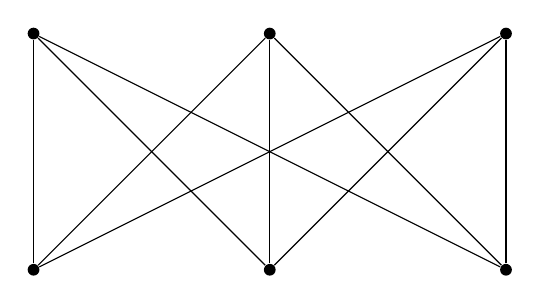
\begin{tikzpicture}[scale=3]
            \node[circle, fill, inner sep=1.5pt] (v1) at (0,0) {};
            \node[circle, fill, inner sep=1.5pt] (v2) at (1,0) {};
            \node[circle, fill, inner sep=1.5pt] (v3) at (2,0) {};
            \node[circle, fill, inner sep=1.5pt] (w1) at (0,1) {};
            \node[circle, fill, inner sep=1.5pt] (w2) at (1,1) {};
            \node[circle, fill, inner sep=1.5pt] (w3) at (2,1) {};
            \draw (v1) -- (w1);
            \draw (v1) -- (w2);
            \draw (v1) -- (w3);
            \draw (v2) -- (w1);
            \draw (v2) -- (w2);
            \draw (v2) -- (w3);
            \draw (v3) -- (w1);
            \draw (v3) -- (w2);
            \draw (v3) -- (w3);

        \end{tikzpicture}
        
        \vspace{1em}
		\scriptsize \(K_{3,3}\)
	\end{column}

	\begin{column}{0.5\textwidth}
		\centering
        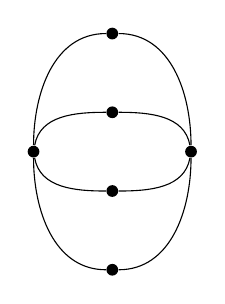
\begin{tikzpicture}[scale=1]

            % Define the two main suspension vertices, positioned closer together
            \node[circle, fill, inner sep=1.5pt] (a1) at (0,0) {};
            \node[circle, fill, inner sep=1.5pt] (a2) at (2,0) {};

            \node[circle, fill, inner sep=1.5pt] (b1) at (1,1.5) {};
            \node[circle, fill, inner sep=1.5pt] (b2) at (1,.5) {};
            \node[circle, fill, inner sep=1.5pt] (b3) at (1,-.5) {};
            \node[circle, fill, inner sep=1.5pt] (b4) at (1,-1.5) {};


    % Draw the edges for the 'm' paths, passing through the b_i nodes
    \draw (a1) to[out=90, in=180] (b1);
    \draw (a1) to[out=80, in=180] (b2);
    \draw (a1) to[out=-80, in=180] (b3);
    \draw (a1) to[out=-90, in=180] (b4);

    \draw (a2) to[out=90, in=0] (b1);
    \draw (a2) to[out=100, in=0] (b2);
    \draw (a2) to[out=-100, in=0] (b3);
    \draw (a2) to[out=-90, in=0] (b4);

        \end{tikzpicture}

        \vspace{1em}
		\scriptsize \(K_{2,4}\)
    \end{column}
\end{columns}
\end{frame}
\begin{frame}{Definitions}
    Given a graph \(\Gamma\), 
\end{frame}
\begin{frame}{A single edge}
\begin{columns}[T,onlytextwidth]
	\begin{column}{0.5\textwidth}
        \vspace{.5em}
		\centering
        \begin{tikzpicture}[scale=3.5]
            \node[circle, fill, inner sep=1.5pt, label=left:\(v\)] (v) at (0,0) {};
            \node[circle, fill, inner sep=1.5pt, label=left:\(w\)] (w) at (0,1) {};
            \draw (v) -- (w);
        \end{tikzpicture}
        
        \vspace{1em}
		\scriptsize \(\Gamma\) is a single edge
	\end{column}

	\begin{column}{0.5\textwidth}
		\centering
        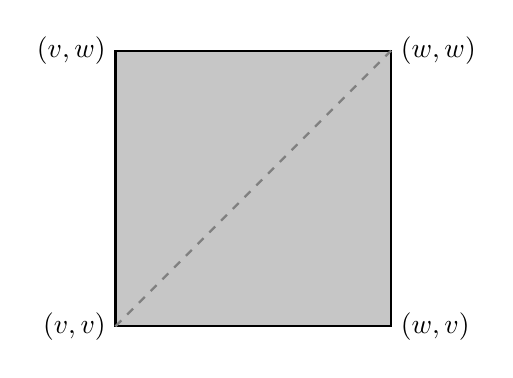
\begin{tikzpicture}[scale=3.5]
            \fill[gray, opacity=0.45] (0,0) rectangle (1,1);
            \draw[thick] (0,0) rectangle (1,1);
            \node[left] (vv) at (0,0) {\((v, v)\)};
            \draw[gray, dashed, thick] (0,0) -- (1,1);
            \node[right] (ww) at (1,1) {\((w, w)\)};

            \node[left] (ww) at (0,1) {\((v, w)\)};
            \node[right] (ww) at (1,0) {\((w, v)\)};
        \end{tikzpicture}

        \vspace{1em}
		\scriptsize \(\Conf_2(\Gamma)\)
    \end{column}
\end{columns}
\end{frame}
\begin{frame}{Two Edges}

\begin{columns}[T,onlytextwidth]
    
	\begin{column}{0.5\textwidth}
        \vspace{5.9em}
		\centering
        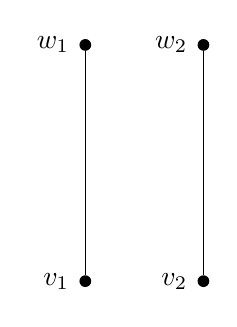
\begin{tikzpicture}[scale=3]
            \node[circle, fill, inner sep=1.5pt, label=left:\(v_1\)] (v1) at (0,0) {};
            \node[circle, fill, inner sep=1.5pt, label=left:\(w_1\)] (w1) at (0,1) {};
            \draw (v1) -- (w1);

            \node[circle, fill, inner sep=1.5pt, label=left:\(v_2\)] (v2) at (0.5,0) {};
            \node[circle, fill, inner sep=1.5pt, label=left:\(w_2\)] (w2) at (0.5,1) {};
            \draw (v2) -- (w2);


        \end{tikzpicture}
        
        \vspace{1em}
		\scriptsize \(\Gamma\) is two disjoint edges
	\end{column}

	\begin{column}{0.5\textwidth}
		\centering
        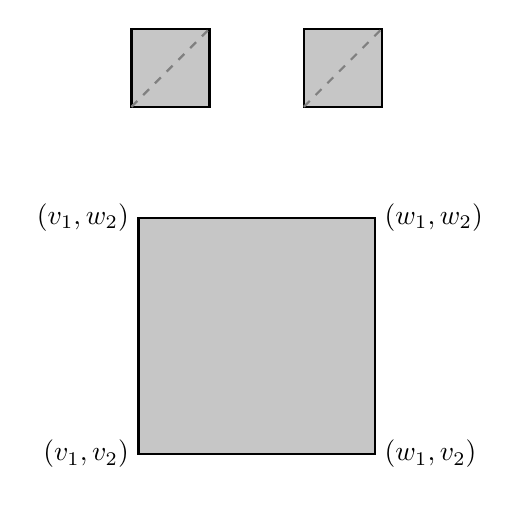
\begin{tikzpicture}[scale=3]

            \fill[gray, opacity=0.45] (0,-.3) rectangle (1,.7);
            \draw[thick] (0,-.3) rectangle (1,.7);
            \node[left] (v1v1) at (0,-.3) {\((v_1, v_2)\)};
            \node[right] (w1w1) at (1,.7) {\((w_1, w_2)\)};
            \node[left] (v1w1) at (0,.7) {\((v_1, w_2)\)};
            \node[right] (w1v1) at (1,-.3) {\((w_1, v_2)\)};


            \fill[gray, opacity=0.45] (-.03,1.5) rectangle (.3, 1.17);
            \draw[thick] (-.03,1.5) rectangle (.3, 1.17);
            \draw[gray, dashed, thick] (-.03,1.17) -- (.3, 1.5);
            %\node[label=above left:{\((v_1,w_1)\)}] (v) at (-.03,1.5) {};
            %\node[label=below right:{\((w_1,v_1)\)}] (w) at (.3,1.17) {};

            \fill[gray, opacity=0.45] (.7,1.5) rectangle (1.03,1.17);
            \draw[thick] (.7,1.5) rectangle (1.03,1.17);
            \draw[gray, dashed, thick] (.7,1.17) -- (1.03,1.5);
            %\node[label=above left:{\((v_2,w_2)\)}] (w) at (.7,1.5) {};
            %\node[label=below right:{\((w_2,v_2)\)}] (w) at (1.03,1.17) {};


        \end{tikzpicture}

        \vspace{1em}
		\scriptsize Part of \(\Conf_2(\Gamma)\).
    \end{column}
\end{columns}

\end{frame}
\begin{frame}{A 3 page book}

\begin{columns}[T,onlytextwidth]
	\begin{column}{0.5\textwidth}
		\centering
        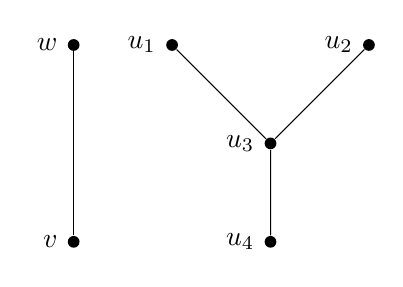
\begin{tikzpicture}[scale=2.5]
            \node[circle, fill, inner sep=1.5pt, label=left:\(v\)] (v) at (0,0) {};
            \node[circle, fill, inner sep=1.5pt, label=left:\(w\)] (w) at (0,1) {};
            \draw (v) -- (w);

            \node[circle, fill, inner sep=1.5pt, label=left:\(u_1\)] (u1) at (0.5, 1) {};
            \node[circle, fill, inner sep=1.5pt, label=left:\(u_2\)] (u2) at (1.5, 1) {};
            \node[circle, fill, inner sep=1.5pt, label=left:\(u_3\)] (u3) at (1, .5) {};
            \node[circle, fill, inner sep=1.5pt, label=left:\(u_4\)] (u4) at (1, 0) {};
            \draw (u1) -- (u3);
            \draw (u2) -- (u3);
            \draw (u3) -- (u4);
        \end{tikzpicture}
			
		\scriptsize \(\Gamma = K_2 \cup K_{1,3}\) 
        
        i.e. \(\Gamma\) is an edge and the ``\(Y\)-graph''.
	\end{column}

	\begin{column}{0.5\textwidth}
		\centering
        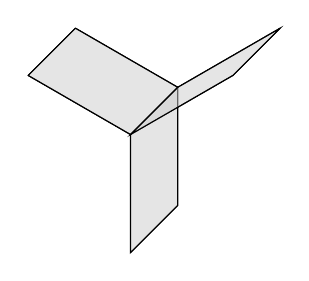
\begin{tikzpicture}[
            scale=1.5,
            x={(1cm,0cm)},
            y={(0cm,1cm)},
            z={(0.4cm,0.4cm)}
        ]

        \coordinate (vu3) at (0, 0, 0);
        \coordinate (wu3) at (0, 0, 1);
        
        \coordinate (vu1) at (-.866, .5, 0);
        \coordinate (vu2) at (0, -1, 0);
        \coordinate (vu4) at (.866, .5, 0);

        \coordinate (wu1) at (-.866, .5, 1);
        \coordinate (wu2) at (0, -1, 1);
        \coordinate (wu4) at (.866, .5, 1);



        % spine
        \draw (vu3) -- (wu3);

        % pages
        \draw (vu3) -- (vu1);
        \draw (vu3) -- (vu2);
        \draw (vu3) -- (vu4);

        \draw (wu3) -- (wu1);
        \draw (wu3) -- (wu2);
        \draw (wu3) -- (wu4);

        \draw (vu1) -- (wu1);
        \draw (vu2) -- (wu2);
        \draw (vu4) -- (wu4);

        % fill in pages as 3D quadrilaterals (one per page) and draw their outlines
        \filldraw[fill=gray!40, fill opacity=0.5, draw=black] (vu3) -- (vu1) -- (wu1) -- (wu3) -- cycle;
        \filldraw[fill=gray!40, fill opacity=0.5, draw=black] (vu3) -- (vu2) -- (wu2) -- (wu3) -- cycle;
        \filldraw[fill=gray!40, fill opacity=0.5, draw=black] (vu3) -- (vu4) -- (wu4) -- (wu3) -- cycle;

        \end{tikzpicture}

		\scriptsize A book is a connected component of \(\Conf_2(\Gamma)\).
    \end{column}
\end{columns}

\end{frame}
\begin{frame}{The Discretized Configuration Space}
    \begin{definition}
        Given a graph \(\Gamma\), a point in the \(n\) point ordered \textit{discretized} configuration space of \(\Gamma\) denoted \(\DConf_n(\Gamma)\)
    is the positions of \(n\) \textit{distinct} particles placed on \(\Gamma\) such that
    no two particles occupy the same vertex or the same edge.
    \end{definition}

    \pause

    Equivalently, \(\DConf_n(\Gamma) = \Gamma^n - \Delta^{\square}\) 
    where \(\Delta^{\square}\) 
    is the ``thick'' diagonal
    \(\{(x_1, \cdots, x_n) \in \Gamma^n \mid x_i \text{ and } x_j \text{ share a cell for some } i \neq j \}\).


    \pause
    \begin{theorem}
        If \(\Gamma\) is sufficiently subdivided, then \(\DConf_n(\Gamma)\) is homotopy equivalent to \(\Conf_n(\Gamma)\)
    \cite{PRUE2014136}.
    \end{theorem}


\end{frame}
\begin{frame}{A single edge (again)}
\begin{columns}[T,onlytextwidth]
	\begin{column}{0.5\textwidth}
        \vspace{.53em}
		\centering
        \begin{tikzpicture}[scale=3]
            \node[circle, fill, inner sep=1.5pt, label=left:\(v\)] (v) at (0,0) {};
            \node[circle, fill, inner sep=1.5pt, label=left:\(w\)] (w) at (0,1) {};
            \draw (v) -- (w);
        \end{tikzpicture}
        
        \vspace{1em}
		\scriptsize \(\Gamma\) is a single edge.
	\end{column}

	\begin{column}{0.5\textwidth}
        \centering
        \begin{tikzpicture}[scale=3]
            % Wrap label text in braces so commas and math-delimiters are handled safely by TikZ
            \node[circle, fill, inner sep=1.5pt, label=right:{\((w,v)\)}] (v) at (1,0) {};
            \node[circle, fill, inner sep=1.5pt, label=left:{\((v,w)\)}] (w) at (0,1) {};
        \end{tikzpicture}

        \vspace{1em}
		\scriptsize \(\DConf_2(\Gamma)\)
    \end{column}
\end{columns}
\end{frame}
\begin{frame}{\(n\)-cubes}

\begin{columns}[T,onlytextwidth]
	\begin{column}{0.5\textwidth}
		\centering
        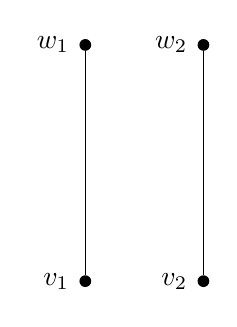
\begin{tikzpicture}[scale=3]
            \node[circle, fill, inner sep=1.5pt, label=left:\(v_1\)] (v1) at (0,0) {};
            \node[circle, fill, inner sep=1.5pt, label=left:\(w_1\)] (w1) at (0,1) {};
            \draw (v1) -- (w1);

            \node[circle, fill, inner sep=1.5pt, label=left:\(v_2\)] (v2) at (0.5,0) {};
            \node[circle, fill, inner sep=1.5pt, label=left:\(w_2\)] (w2) at (0.5,1) {};
            \draw (v2) -- (w2);


        \end{tikzpicture}
        
		\scriptsize \(\Gamma\) is two disjoint edges.
	\end{column}

	\begin{column}{0.5\textwidth}
		\centering
        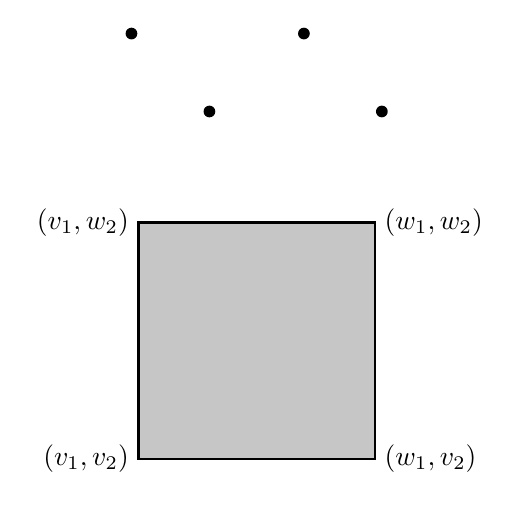
\begin{tikzpicture}[scale=3]
            \fill[gray, opacity=0.45] (0,-.3) rectangle (1,.7);
            \draw[thick] (0,-.3) rectangle (1,.7);
            \node[left] (v1v1) at (0,-.3) {\((v_1, v_2)\)};
            \node[right] (w1w1) at (1,.7) {\((w_1, w_2)\)};
            \node[left] (v1w1) at (0,.7) {\((v_1, w_2)\)};
            \node[right] (w1v1) at (1,-.3) {\((w_1, v_2)\)};


            \node[circle, fill, inner sep=1.5pt] (v1w1) at (-.03,1.5) {};
            \node[circle, fill, inner sep=1.5pt] (w1v1) at (.3,1.17) {};
            \node[circle, fill, inner sep=1.5pt] (v2w2) at (.7,1.5) {};
            \node[circle, fill, inner sep=1.5pt] (w2v2) at (1.03,1.17) {};
        \end{tikzpicture}

		\scriptsize \(\DConf_2(\Gamma)\).
    \end{column}
\end{columns}

\end{frame}
\begin{frame}{\(\DConf_2(K_5)\) is a surface}

\begin{columns}[T,onlytextwidth]
	\begin{column}{0.5\textwidth}
		\centering
        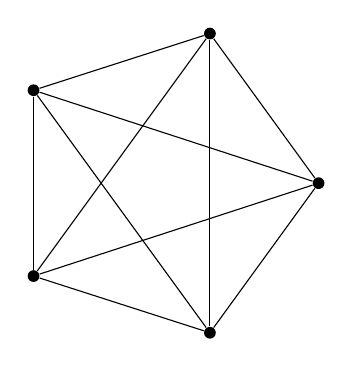
\begin{tikzpicture}[scale=2]
            \node[circle, fill, inner sep=1.5pt] (v1) at (1, 0) {};
            \node[circle, fill, inner sep=1.5pt] (v2) at (.31, .95) {};
            \node[circle, fill, inner sep=1.5pt] (v3) at (-.81, .59) {};
            \node[circle, fill, inner sep=1.5pt] (v4) at (-.81, -.59) {};
            \node[circle, fill, inner sep=1.5pt] (v5) at (0.31,  -0.95) {};
            
            \draw (v1) -- (v2);
            \draw (v1) -- (v3);
            \draw (v1) -- (v4);
            \draw (v1) -- (v5);
            \draw (v2) -- (v3);
            \draw (v2) -- (v4);
            \draw (v2) -- (v5);
            \draw (v3) -- (v4);
            \draw (v3) -- (v5);
            \draw (v4) -- (v5);
        \end{tikzpicture}
        
        \vspace{1em}
		\scriptsize \(K_5\)
	\end{column}

	\begin{column}{0.5\textwidth}
		\centering
        \vspace{9.5em}
        \url{https://skfb.ly/AYo8}

		\scriptsize

        \vspace{1em}
        Michelle Chu's model of \(\DConf_2(K_5)\)
    \end{column}
\end{columns}
\end{frame}
\begin{frame}{Other surfaces?}
    \begin{block}{Theorem (\cite{abrams2000configurationspaces})}
    \(\DConf_{n}(\Gamma) \cong \DConf_{V(\Gamma) - n}(\Gamma)\) 
    \end{block}
    \pause
    \begin{itemize}
        \item \(\DConf_2(K_5) \cong \DConf_3(K_5)\)
        \pause

        \item Abrams also showed that \(\DConf_2(K_{3,3}) \cong \DConf_4(K_{3,3})\) is a surface.
        \pause
    
        \item \(\DConf_3(K_{2,4})\) is a surface (\cite{ko2012characteristics}).
    \end{itemize}
\end{frame}
\begin{frame}{Ruling out graphs}
    \begin{block}{Proposition (W 2025)}
    If \(\DConf_n(\Gamma)\) were a connected \(m\)-manifold without boundary,
    then \(\DConf_n(\Gamma)\) would have to be exactly one of the following:
    \begin{itemize}
        \pause
        \item \(\DConf_{m}(K_{2m+1}) \cong \DConf_{m+1}(K_{2m+1})\) 
        \pause
        \item \(\DConf_{m}(K_{m+1,m+1}) \cong \DConf_{m+2}(K_{m+1, m+1})\)
        \pause
        \item \(\DConf_{m+1}(K_{m,m+2})\)
    \end{itemize}
    \end{block}

    \pause
    If \(m=2\) these align with the known surfaces. 
    
    However, \(\DConf_m(K_{2m+1})\) and \(\DConf_m(K_{m+1,m+1})\) are not \(m\)-manifolds for \(m \geq 3\) (\cite{abrams2000configurationspaces})

    
\end{frame}
\begin{frame}{Open Questions}
     \begin{itemize}
        \item[\(\bullet\)] For what \(\Gamma\) and what \(n\) is \(\DConf_n(\Gamma)\) a manifold? (\cite{abrams2000configurationspaces})
        \item[\(\bullet\)] What are the formulae for higher homology groups of \(\DConf_n(\Gamma)\)? (\cite{ko2012characteristics})
        \item[\(\bullet\)] What is \(\pi_1(\DConf_n(K_{2,m}))\)? (\cite{Berlyne2023})
     \end{itemize}
\end{frame}
\begin{frame}{Applications}
    Configuration spaces of graphs can be used to model:
    \begin{itemize}
        \item Robots moving along a factory floor (\cite{ghrist1999configurationspacesbraidgroups}).
        \item Anyon dynamics in quantum computers (\cite{Maciazek2019}).
        \item Fluids in digital microfluidic devices (\cite{GHRIST2007302})
    \end{itemize}

\end{frame}
\begin{frame}

\centering
Thank you!
\end{frame}

\begin{frame}[allowframebreaks]{References}
  \printbibliography
\end{frame}

\end{document}
